\documentclass[conference]{IEEEtran}
\IEEEoverridecommandlockouts
% The preceding line is only needed to identify funding in the first footnote. If that is unneeded, please comment it out.
\usepackage{cite}
\usepackage{amsmath,amssymb,amsfonts}
\usepackage{algorithmic}
\usepackage{graphicx}
\usepackage{textcomp}
\usepackage{xcolor}
\usepackage{amsmath}
\def\BibTeX{{\rm B\kern-.05em{\sc i\kern-.025em b}\kern-.08em
    T\kern-.1667em\lower.7ex\hbox{E}\kern-.125emX}}
\begin{document}

\title{Optimization in Energy and Power\\
{\footnotesize Group 41 (AI2101- CONVEX OPTIMIZATION)}
% \thanks{Identify applicable funding agency here. If none, delete this.}
}

\author{

 Kunal Nema\\\emph{MA20BTECH11007}\\ 
\and Sparsh Gupta\\ \emph{MA20BTECH11015}\\ 
\and Varunaditya  Singhal\\ \emph{MA20BTECH11021}\\ 
\and Prakhar Patni \\ \emph{MA20BTECH11014}\\ 
}



\maketitle

\begin{abstract}
This project explore the idea of solving the energy management problem for hybrid electric vehicles (HEVs) with engine start and gear shift costs. The control of the power flow among different power devices is commonly referred to as energy management. Here our target is to converge to the globally optimal solution while still being computationally efficient. Using convex optimization along we can reach our desired result in less time. We will use method which can handles state constraints and also allows us to deal with the scenarios where the battery state of charge (SOC) reaches its boundaries.
\end{abstract}

\begin{IEEEkeywords}
HEV, energy management, convex optimization
\end{IEEEkeywords}

\section{\textbf{Introduction}}
Hybrid vehicles consist of generally two power sources, an internal combustion engine and one or more electricity-powered motors, as well as an energy buffer which is usually a Battery. \\
 Energy management via Heuristic approaches and optimization based approaches gives the best result. Our ultimate aim is to construct an optimal energy management control. Applying optimization-based methods for the energy management of parallel hybrid vehicles without penalizing engine start or gearshift events can lead to unacceptably frequent engine starts and gearshifts, eventually leading to an increased fuel consumption, excessive wear of components and/or an uncomfortable driving experience. \\
 Thus, The inherent decision variables which are engine start and gear shift are identified using DP and heuristic approximations which is assumed to be given for our convex problem formulation. \\
The report is structured as follows:

\section{\textbf{Vehicle Model}}

\subsection{Introduction to Convex Vehicle Modeling}
The very first task is that the generic, nonlinear vehicle model
has to be approximated by a convex model, for a general introduction to convex optimization, and for an introduction to convex modeling and optimization of HEVs.\\
A convex description of our model requires the component models to be expressed as a convex function of the free optimization variables which are used by the convex solver. Examples of such free optimization variables are the torques of the motor and the engine, the electrical power consumption of the motor, the fuel consumption, the battery current and the battery state of charge (SOC).
For our study we restricted our count of decision variables till 3. The engine on/off, the gear, and the torque split between the engine and the motor.Since the engine on/off and the gear decision are inherently discrete, these variables are assumed to be known prior to solving a convex optimization problem. The only convex decision variable is the torque split.\\
All vehicle parameters are listed in Table 1.\\
\textbf{Table 1.} Parameters of the pre-transmission parallel HEV (Data Set)

\begin{center}
% \begin{array}{ l c c } 
\begin{tabular}{ c c c }  
\hline
\textbf{Parameter} & \textbf{Symbol} & \textbf{Value} \\
\hline
% \begin{math}
Wheel radius & $r_{w}$  & 0.32 m \\
 \text{Air density} & $\rho_{air}$ & 1.24 $kg/m^3$ \\
 Effective frontal area & $c_d \cdot A$ & 0.60 $m^2$ \\
 Rolling friction coef. & $c _r$ & 0.012 \\
 Gravit. constant & $a_g$ & 9.81 $m/s^2$ \\
 Total vehicle mass & $m_v,1$ & 800 kg\\
 Rot. equiv. mass (gear-dep.) & $m_r$ & [129,84,72,61,55,52,51] kg \\
 Gear ratios & $i_g$ & [10.8,7.1,4.7,3.4,2.5,2.0,1.8]\\
 Gearbox efficiency param. & $\eta_{g,0}$ & 0.95 \\
 Gearbox efficiency param. & $\eta_{g,1}$ & 0.02 1/(rad/s) \\
 Gearbox efficiency param. & $\omega_{g,1}$ & 400 rad/s \\
 Nominal motor power &  & 40 kW \\
 Max. motor speed & $\omega_{m,max}$ & 628 rad/s \\
 Nominal engine power &  & 150 kW \\
 Min. engine speed & $\omega_{e,min}$ & 105 rad/s \\
 Max. engine speed & $\omega_{e,max}$ & 628 rad/s \\
 Max. battery capacity & $Q_0$ & 7.64 A h \\
 Open circuit voltage & $V_{oc}$ & 263 V \\
 Battery int. & resistance $R_i$ & 0.24 $\omega$ \\
 Min. battery current & $I_{b,min}$ & -200 A \\
 Max. battery current & $I_{b,max}$ & 200 A \\
 Min. SOC & $SOC_{min}$ & 0.20 \\
 Max. SOC & $SOC_{max}$ & 0.80 \\
 Aux. power demand & $P_{aux}$ & 400 W  \\

\hline
\end{tabular}
\end{center}

\subsection{Road Load Model}

\begin{figure}[h]
    \centering
    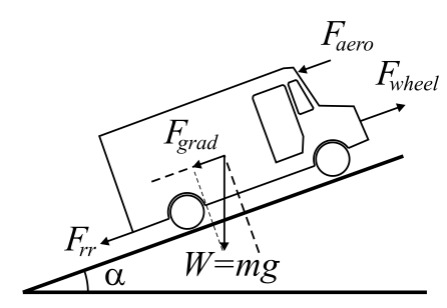
\includegraphics[scale = 0.45]{road load model.jpeg}
    \caption{Vehicle Model}
    \label{fig:}
\end{figure}

For this model of the vehicle we assume that its in quasi-static state, with velocity $v$, acceleration $a$ and at a slope of the road $\alpha$. At at a particular time k $\in$ $\mathbb{N}$ ,we so wheel speed $w_w$ can be given by:
\begin{equation}\label{eq1}
w_w(k) = \frac{v(k)}{r_w}
\end{equation}

We can calculate wheel torque $(T_w)$ from wheel radius ($r_w$) and Net Force ($F_{net}$):
\[T_w(k) = r_w \cdot (F_{net})
\]
The forces which act on the vehicle in its moving state are: \\
\[F_{aero} = \frac{1}{2}\rho_{air}c_d Av^2(k)b
\]
\[F_{rr} = c_r m_v a_g  cos(\alpha(k))
\]
\[F_g = m_v a_g sin(\alpha(k))
\]
\[F_{wheel} = m_v + m_r(g(k))) a(k)
\]

Thus the Net Force ($F_{net}$) can be given by \\
\[ \Rightarrow F_{net} = F_{aero} + F_{arr} + F_g + F_{wheel}
\]

Therefore wheel torque $(T_w)$ is defined by:
\vspace{-6pt}
\begin{multline}
T_w(k) = r_w \cdot (\frac{1}{2}\rho_{air}c_d Av^2(k)b + c_r m_v a_g  cos(\alpha(k)) + \\m_v a_g sin(\alpha(k))  + (m_v +m_r(g(k))) a(k))
\end{multline}
Note that $m_r$ depends on the choice of the gear.

\vspace{10pt}
\subsection{Gearbox Model}
In this model, we derive expressions for gearbox speed and torque which depend on gear ratio. \\

The tangential speed is the same in the contact point of the two gears (also represented in the Fig 2). \\

The tangential speed ($v_t$) is the product between the radius and the rotational speed and thus we can write: \\

\[
w_g \cdot r_{in} = v_t = w_w \cdot r_{out} \quad \text{and}
\]
since
\[ \frac{r_{out}}{r_{in}} = i_g
\]

We can define gearbox speed ($w_g$) as :
\begin{equation}\label{eq1}
w_g(k) = w_w(k) \cdot i_g(k)
\end{equation}


\begin{figure}[h]
    \centering
    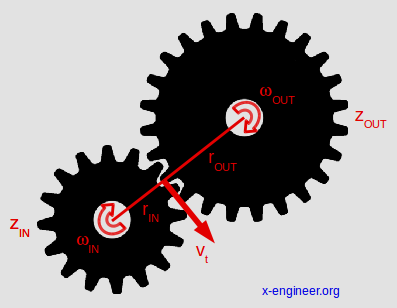
\includegraphics[scale = 0.45]{gearbox model.png}
    \caption{Effect of the gear ratio on the output speed}
    \label{fig:}
\end{figure}

The relationship between the output torque and the input torque is the following:
\[T_g = T_w \cdot \frac{1}{i_g(k)} \cdot ({\eta_{net}})
\]

We define the gearbox torque ($T_g$) as follows:

\begin{multline}
T_g(k) = T_w(k) \cdot \frac{1}{i_g(k)} \cdot {(\eta_{g,0} - \frac{\eta_{g,1}}{\omega_{g,1} } \cdot \omega_g(k))^{-sign(T_w(k)}}
\end{multline}

\textbf{Moreover, losses occurring during gearshifts are assumed to consume $m_g$ = 0.01 g fuel equivalent
per gearshift},i.e
\begin{equation}\label{eq1}
m_g(k)= \begin{cases}
    0.01 & \text{if } g(k)\neq g(k-1)\\
    0              & \text{otherwise}
\end{cases}
\end{equation}

The gear $g$ is being controlled by gear controlled variable $u_g$ (which comes as one of the result of DP):
\begin{equation}\label{eq1}
g(k)= g(k-1) +u_g(k), \quad u_g \in \{-1,0,1\}
\end{equation}

\subsection{Torque Split Model}
The torque split between the electric motor and the internal combustion engine is determined by the
motor torque $u_{ts}$ $\equiv$ $T_m$ such that the engine torque $T_e$ is determined by:
\begin{equation}
    T_e(k) = T_g(k) - u_{ts}(k)
\end{equation}
This equation is convex in any of the variables involved.


\subsection{Electric Motor Model}
For our project we assumed the nominal power of the electric motor to be 40kW, along with the assumption that the motor is coupled with the gearbox, thus the $w_m = w_g$, i.e velocity of motor is equal to velocity of the gearbox.\\
The power of the electric motor is being approximated for a $2^{nd}$ degree polynomial of $T_m$, with speed dependent coefficients, taking time(k) as constant.


\begin{equation}\label{eq1}
    P_m \geq b_0(\omega_m) + b_1(\omega_m)T_m + b_2(\omega_m)T^2
\end{equation}

The equation is convex with description $T_m$, even though we say that the equation is not optimal and waste energy , but in our optimal case the equality holds. \\
The working of the motor is limited by its max and min torque limitations, as well as by its max speed:
\begin{equation}\label{eq1}
    0 \leq \omega_m(k) \leq \omega_{m,max}
\end{equation}
\begin{equation}\label{eq1}
   T_{m,min}(\omega_m(k)) \leq T_m(k) \leq T_{m,max}(\omega_m(k)) 
\end{equation}
The following figure 3 depicts the relation of $P_m$ with different values of $T_m$ , keeping  25 kW permanent magnet synchronous motor.\\
We can clearly observe that the equation is convex with respect to $T_m$\\
\begin{figure}[h]
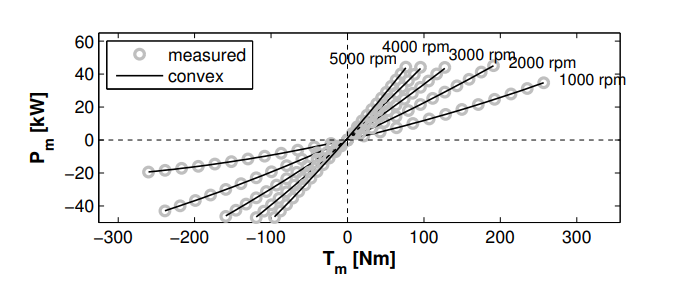
\includegraphics[width=9cm]{Electric Motor graph.png}
\caption{Convex motor model}
\end{figure}
\subsection{Engine Model}

The mass flow $\dot{\textit{\textbf{m}}}_f$ of the fuel consumed is approximated by a second-order polynomial with
speed-dependent coefficients (for all times i.e., neglecting time index k):
\begin{equation}
    \dot{\textit{\textbf{m}}}_f(k) \geq u_e(k)\cdot (a_0&(k)+a_1(k)\cdot \textbf{T}_e{k}+a_2(k)\cdot \textbf{T}_e^2(k))
\end{equation}
where is $w_e$ denotes rotational speed of the engine. 

This above mentioned equation is convex in the variable $T_e$. \\


At all times, the engine is only allowed to operate within its limits defined by a maximum torque, minimum speed and a maximum speed condition which can be represented with constraints:
\begin{equation}
    w_{e,min} \leq w_e(k) \leq w_{e,max}
\end{equation}

\begin{equation}
    0 \leq T_e(k) \leq T_e(w_e(k))
\end{equation}

\begin{figure}[h]
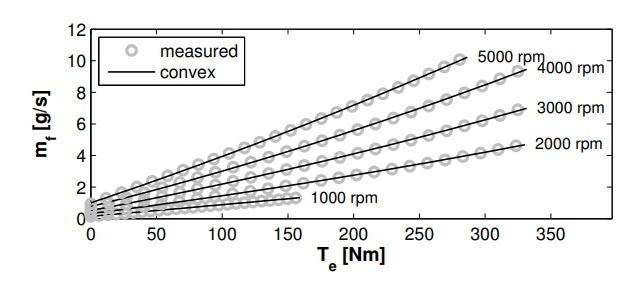
\includegraphics[width=9cm]{engine model.jpeg}
\caption{Convex engine model}
\end{figure}



The measurement data were obtained for a modern 125 kW turbocharged spark-ignited combustion engine. The torque axis is then linearly scaled with the nominal power while the efficiencies are kept constant.The engine on/off decision is determined via the variable $u_e \in \{0, 1\}$ such that the engine state e is dictated by:
\begin{equation}
    e(k) = u_{e}(k)
\end{equation}

here, the value e = 1 represents the “on” state; and e = 0 represents the “off” state. If the engine is on, the engine speed is equal to $w_g$, unless the first gear is engaged, where the clutch is allowed to slip. If the engine is off, the engine speed is equal to zero, and the engine is disconnected from the rest of the powertrain. Moreover, each engine start is assumed to consume me = 0.3 g fuel equivalent, i.e., 

\begin{equation}\label{eq1}
m_e(k)= \begin{cases}
    0.3 g & \text{if } e(k) = 1 \text{ and } e(k-1) = 0\\
    0              & \text{otherwise}
\end{cases}
\end{equation}

These start costs represent the fuel-equivalent costs to start the engine. In the optimization, artificial costs can be assigned in order to reduce frequent engine starts.

\subsection{Battery Model}
The actual model is a non-linear model where the open circuit voltage is a function of State of Charge(SOC).\\
For our project we modelled it as convex , with open circuit voltage $V_{oc}$ in series and a constant resistance $R_i$. These assumptions are reasonable in the operating range of the battery.\\
The figure 5 explains it more clearly\\
\begin{figure}[h]
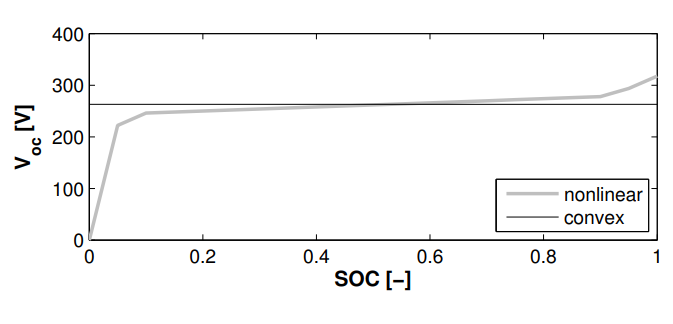
\includegraphics[width=9cm]{Voltage model .png}
\caption{Non linear model V/S Approximated model of Open circuit voltage of the battery}
\end{figure}
In our convex case the dynamics of the battery State of Charge (SOC) are as follows:\\
\begin{equation}\label{eq1}
   SOC(k + 1) = SOC(k) - \Delta t \cdot \frac{I_b(k)}{Q_0}
\end{equation}
\begin{equation}\label{eq1}
   I_b(k) = \frac{V_{oc} −\sqrt{V_{oc}^2- 4 R_i(P_m(k)+P_{aux})}}{2 \cdot R_i} 
\end{equation}
\begin{itemize}
    \item $I_b$ is the battery current.
    \item $P_{aux}$ is a constant power consumed by electric auxiliary units.
    \item $\Delta$ t is the sampling time = 1 sec.
\end{itemize}
Equation 16 is convex , but the equation 17 need to be formulated as:\\
\begin{equation}\label{eq1}
  P_m(k) \leq V_{oc} \cdot I_b(k) − R_i \cdot I^2_b(k) − P_{aux} 
\end{equation}
In order to maintain the convexity the variable of interest and battery SOC are being constraint as follows:
\begin{equation}\label{eq1}
  I_{b,min} \leq I_b(k) \leq I_{b,max} 
\end{equation}
\begin{equation}\label{eq1}
  SOC_{min} \leq SOC(k) \leq SOC_{max} 
\end{equation}

 



\subsection{Overview}
The control variable $u$ and the states $x$ of the system are as follows:\\
\begin{equation}
 u(k) = \begin{bmatrix}
\begin{matrix} u_g(k) \\ u_e(k) \\ u_{ts}(k) \end{matrix} 
\end{bmatrix}
\end{equation}
\begin{equation}
 x(k) = \begin{bmatrix}
\begin{matrix} SOC(k) \\ g(k) \\ e(k) \end{matrix} 
\end{bmatrix}
\end{equation}

\section{\textbf{Problem Formulation}}
The problem to be solved is the energy management problem formulated as an optimal control problem as follows: \\
(Note: variables depending on Gear-shift and Engine On/Off aren't being minimized using Convex Optimization but will be handled by DP separately)
\begin{equation}
\min_{k\leq N}  \sum_{k=1}^N \dot{\textbf{m}}_f(k).\Delta t
\end{equation}

Subject to all equations presented in vehicle model and the charge-sustenance condition $SOC(N + 1) = SOC(1) = SOC_{0}$ with $SOC_{0}$ being the initial state of charge.\\
The energy management problem can be solved using DP. However, to account for the engine start
and gearshift losses, three state variables are required, i.e., the battery SOC, the engine state, and the
gear currently engaged. Unfortunately, the computation time of this pure DP approach is large even
for a coarse discretization for the SOC. Moreover, the accuracy of the solution is influenced by the
discretization of the problem.\\
As such, DP optimizes the equivalent fuel
consumption for a given equivalence factor and for given engine start and gearshift costs, and the optimal
solution is found by iterating on the equivalence factor until a charge sustaining solution is found.
Its main drawback is the fact that finding a charge-sustaining equivalence factor
cannot be guaranteed, and therefore a heuristic approach has to be used instead.\\
\textbf{Convex optimization} is used to find a charge-sustaining equivalence factor and to handle the state
constraints, while DP is used to find the optimal engine on/off and gearshift strategy.\\

\emph{We will be dealing with the convex optimization problem formulation and solution of it for our project.}
\section{\textbf{Iterative Algorithm}}

\emph{s} denotes the equivalence factor between fuel consumption and electrical energy consumption.

This equivalence factor is basically the Lagrange multiplier of the Euler-Lagrange formulation of the
optimal control problem, sometimes also referred to as the dual variable.
The equivalence factor is determined solving the convex optimization problem.\\
The convex optimization problem to be solved is formulated as follows (bold symbols represent optimization variables):\\
Minimize:

\begin{subequations}
\begin{equation}
    \sum_{k=1}^{N} \dot{\textit{\textbf{m}}}_f(k) \cdot \Delta t \label{eq:obj}
\end{equation}
Subject To:
\begin{align}
    \textbf{P}_m{k} \leq V_{oc} &\cdot \textbf{I}_b(k) - R_i\cdot \textbf{I}_{b}^2(k) - P_{aux} \\
    \dot{\textit{\textbf{m}}}_f(k) \geq u_e(k)\cdot (a_0&(k)+a_1(k)\cdot \textbf{T}_e{k}+a_2(k)\cdot \textbf{T}_e^2(k) ) \\
    T_g(k) &= \textbf{T}_m(k)+u_e(k)\cdot \textbf{T}_e(k) \\
    \textbf{P}_m(k) \geq b_0(k)+&b_1(k)\cdot \textbf{T}_m(k)+b_2(k)\cdot \textbf{T}_m^2(k) \\
    \textbf{SOC}(k+1) &= \textbf{SOC}(k) - \Delta t\cdot \frac{\textbf{I}_b(k)}{Q_0} \\
    \textbf{T}_m(k) &\geq T_{m,min}(k) \\
    \textbf{T}_m(k) &\leq T_{m,min}(k) \\
    \textbf{T}_e(k) &\geq 0 \\
    \textbf{T}_e(k) &\leq T_{e,max}(k) \\
    \textbf{I}_b(k) &\geq I_{b,min} \\
    \textbf{I}_b(k) &\leq I_{b,max} \\
    \textbf{SOC}(k) &\geq SOC_{min} \\
    \textbf{SOC}(k) &\leq SOC_{max} \\
    \textbf{SOC}(1) &= SOC_0 \\
    \textbf{SOC}(N+1) &= SOC_0
\end{align}
\end{subequations}
for all $k \in \{1,2,...,N\}$

Note that the gearshift and engine on/off sequence must be defined prior to solving Convex problem, otherwise the problem is not convex. As a consequence, the gearbox torque and the speeds $T_{g}(k)$ and the speeds $\omega_{e}(k)$ and $\omega_{g}(k)$ can be precalculated for the entire driving cycle.

From the above illustrated figure, we are being $s_{in}$, s.t. $s_{in}(k) \forall k \in \{1,...,N\}$ (and the optimal value which we get for $s_{in}$ through the model be $s^*$) as the input for the DP component of our model, for that $s_{in}$ we wish to get the optimal values for $u_e$ and $u_g$, which can also be written as $u_e \equiv u_e^*$ and $u_g \equiv u_g^*$. Later, we use these optimal values for finding $s_{out}$ or optimal fuel consumption i.e., $s^*$, hence $s_{out} \equiv s^*$.\\

\begin{figure}[h]
    \centering
    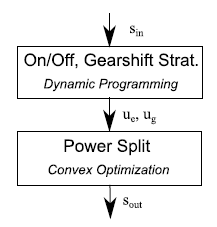
\includegraphics[]{Sequential.png}
    \caption{Sequential Model for Algorithm}
    \label{fig:seq}
\end{figure}

A necessary condition for optimality of my model is if $'s_{in} \equiv s^{*}'$, then $'s_{in} \equiv s_{out} '$ because we know indeed the output of our sequential model (i.e. $s_{out}$) is also the optimal solution for given $s_{in}$ which is $s^{*}$.\\
To derive the sufficiency of condition only if $'s_{in} \equiv s_{out}'$, then $'s_{out} \equiv s^*'$, we need to consider 2 further cases where $s_{in} \not\equiv s^*$. First, if we are getting optimal values of $u_e$ and $u_g$ even-though $s_{in} \not\equiv s^*$ (this may happen if any of any of our constraints for DP don't guarantee optimality) and second case, if $u_e \not\equiv u_e^*$ or $u_g \not\equiv u_g^*$, we might get $s_{out} \not\equiv s^*$, and also $s_{in} \not\equiv s_{out}$. \\

Hence, the solution results in an energy management strategy (i.e., $u_ts, u_g, u_e$) in which the vehicle is operated in the pure electric mode for more time, implying also that the engine is used less than in the optimal solution. “Using the engine less” means that recharging the battery via operating point shifting is done at
lower additional loads than optimal, but also that the total engine run-time is less than optimal. Therefore, the SOC is not sustained over the entire driving cycle.

Therefore, if and only if $s_{in} \equiv s_{out}$, then $s_{out} \equiv s^*$. Now, by using this condition we devise a iterative model over our sequential model to get output as the optimal value:
\begin{figure}[h]
    \centering
    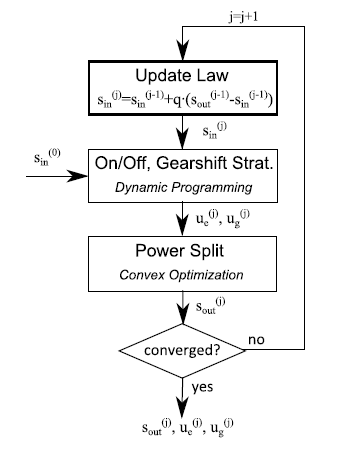
\includegraphics[scale = 0.5]{Iterative.png}
    \caption{Iterative Sequential Model}
    \label{fig:Iterseq}
\end{figure}

Details of steps in the iterational model:\\
\textbf{Step 1: Initialization of the Algorithm}\\
The iteration counter is initialized by $j = 0$. The initial equivalence factor $s_{in}^{(0)}$
in is initialized by a constant value for the entire driving cycle.


\noindent\textbf{Step 2: Use of DP to obtain $u_g^{(j)}, u_e^{(j)}$}\\
In this step, based on $s_{in}^{(j)}$ in , DP is employed to give off optimal $u_g$ and $u_e$. Notice that in total only two states are needed, namely one for the gear and one for the engine on/off state. A state for the battery SOC is not included. As a result, new values of $u_g^{(j)}$ and $u_e^{(j)}$ are obtained which are optimal for $s_{in}^{(j)}$.

\noindent\textbf{Step 3: Use of convex optimization to obtain $s_{out}^{(j)}$}\\
For the acquired values of $u_g^{(j)}$ and $u_e^{(j)}$, we calculate the $s_{out}$ by solving the convex optimization problem in \ref{eq:obj}.

\noindent\textbf{Step 4: Check for Convergence}\\
As we already showed that the solution shall be optimal (or will be acquired) \emph{if and only if} $s_{in}^{(j)} \equiv s_{out}^{(j)}$, hence we calculate the root mean square error with a predefined tolerance $E_{Tol}$ and check if our error $E$ is larger then $E_{Tol}$ we increase $j \rightarrow j+1$ and update law as in Step 5. If $E$ is less than $E_{Tol}$ it \emph{converges}
.\begin{equation}
    E = \sqrt{\frac{1}{N}\sum_{k=1}^N(s_{in}(k)^{(j)} - s_{out}(k)^{(j)})^2}
\end{equation}
\noindent\textbf{Step 5: Update law}\\
Performing Steps 2 and 3 does not necessarily yield the optimal solution since the optimal equivalence factor is unknown. Initializing the equivalence factor $s_{in}$ with a too high value will result in a too low value for $s_{out}$ (and vice versa), as explained above. Therefore, the optimal $s^*$ lies between $s_{in}$ and $s_{out}$. To ensure convergence towards $s^*$, damping is introduced by including an update law for the equivalence factor $s_{in}^{(j)}$ in before step 2.
\begin{equation}
    s_{in}^{(j)} = s_{in}^{(j-1)} + q\cdot (s_{out}^{(j-1)} - s_{in}^{(j-1)}
\end{equation}
Here $q$ is the convergence parameter and its value initially is taken as $q = 0.2$, also whenever the error $E$ is larger $E_{Tol}$ our convergence parameter is reduced by $q \rightarrow 0.7 \cdot q$. Using this update law, $s_{out}^{(j)}$ will convergent to $s^*$ for a $j$ as $j \rightarrow \infty$.

\section{\textbf{Results}}
The minimum and maximum values of the SOC are assumed to be $20\%$ and $80\%$, respectively. 
The given table summarizes the fuel consumption, the number of engine starts, the number of gearshifts, and the computation time for the four cases considered.

\begin{center}
\begin{tabular}{ c c c c }  
\hline
\textbf{Cycle} & \textbf{Performance Index} & \textbf{DP} & \textbf{DP-C} \\
\hline
% \begin{math}
NEDC & FC[L/100 km]  & 4.405 & 4.399 \\
  & ICE starts [\#] & 7 & 7 \\
 & Gearshifts [\#] & 86 & 86 \\
&CPU time [s] & 791 & 6 \\
\hline
FTP &FC [L/100 km] &4.288 &4.279\\ 
&ICE starts [\#] &28 &28 \\
&Gearshifts [\#] &180 &182 \\
&CPU time [s]& 1287 &14 \\
\hline
CADC &FC [L/100 km] &5.635 &5.627 \\
&ICE starts [\#] &78 &75 \\
&Gearshifts [\#] &316 &310 \\
&CPU time [s] &2363 &105 \\
\hline
CADC &FC [L/100 km] &5.657 &5.643\\ 
(bounded) &ICE starts [\#] &90 &85 \\
&Gearshifts [\#] &322 &310 \\
&CPU time [s]  &527 &122 \\

% \end{math}
\hline
\end{tabular}
\end{center}

Comparing the computational burden associated with the DP-C and the DP methods, the DP-C significantly outperforms the DP method. As the table shows, the DP-C method requires less than 10\% of the time required by the DP method. In the case of the “CADC bounded”, the DP-C method still requires only about 20\% of the time required by the DP method, although a reduced number of discrete supporting points for the SOC state are used in the DP method. \\

Summarizing the findings described in this section, the DP-C method yields more accurate results in much less time than a pure DP implementation.

\section{\textbf{Discussion}}

\noindent\emph{Advantages and disadvantages of the DP-C method.}
A substantial advantage of the DP-C method is its ability to yield globally optimal results for the convex vehicle model much faster than the DP method. Moreover, the equivalence factor related to the battery state is obtained directly from the convex solver without any error-prone calculation via the
optimal cost-to-go from DP. Furthermore, more accurate results can be obtained with the DP-C method than with the DP method because no discretisation of the SOC state is necessary. In addition, DP-C is also able to handle state constraints, which means that it detects the jumps in the equivalence factor.

The only drawback of the DP-C method are the modeling errors introduced by the convex modeling of the powertrain. However, in the case of the HEV in this paper, the errors are small.

\section{\textbf{Conclusions}}

This paper presents a method to calculate the globally optimal energy management strategy for a parallel HEV on a given driving cycle taking into account penalties to avoid frequent engine start and/or gearshift events. The proposed method combines DP and convex optimization in an iterative scheme.
The algorithm converges to the globally optimal solution after a few iterations. The optimal gearshift and engine on/off strategy was in advance evaluated while convex optimization is used to determine the optimal power split strategy. The proposed method delivers globally optimal results with respect to the convex vehicle model, even in the presence of state constraints. The proposed method results in a substantial reduction of the evaluation time.

For the convex vehicle model, the proposed method delivers a higher precision than DP (0.1\%–0.2\% lower fuel consumption) while incurring significantly less computational effort (75\%–98\% less). The higher precision is due to the fact that convex optimization does not require a discretization of the
continuous control and state variables, which inherently introduces interpolation errors. To evaluate the magnitude of the error that is introduced by using convex model approximations, the strategy that
was optimized for the convex model is applied to the nonlinear model. Compared to the true globally optimal solution obtained by applying DP on the nonlinear model, the proposed method results in a slight deterioration of precision only (up to 0.3\% increased fuel consumption).

The proposed method can be extended to other vehicle topologies and different formulations of the energy management problem. For example, the battery state of health or the engine temperature could be considered by including further continuous state variables. Additional discrete state variables, such
as for example the clutch state, as well as additional continuous and discrete control variables, such as for example the desired clutch state, the motor speed or torque of a series-parallel hybrid vehicle, could be included as well.


\section*{Acknowledgment}
The authors express their sincere gratitude to Aditya Siripuram Sir for being our instructor for the course and giving us this project.
\begin{thebibliography}{00}
\bibitem{b1} Convex Optimization for the Energy Management of Hybrid Electric Vehicles Considering Engine Start and Gearshift Costs \\ \textbf{Authors}: Tobias Nuesch *, Philipp Elbert, Michael Flankl, Christopher Onder and Lino
Guzzella (Institute for Dynamic Systems and Control) \\
\textbf{Published}: 19 February 2014
\bibitem{b2} IEEE Transactions on Vehicular Technology ( Volume: 63, Issue: 8, Oct. 2014)
\bibitem{b3} Boyd, S.P.; Vendenberghe, L. Convex Optimization; Cambridge University Press: New York, NY, USA, 2004.
\bibitem{b4} Optimization of hybrid energy systems and adaptive energy management for hybrid electric vehicles by Achikkulath Prasanthi,  aHussain Shareefa, Madathodika Asnaa Ahmad Asrul Ibrahimb Rachid Errouissia

\end{thebibliography}

\end{document}
